\chapter{Entwurf einer Bewertungsmatrix}
\label{ch:matrix}

Um die verschiedenen CAPTCHA-Arten bewerten zu können, muss eine Bewertungsmatrix entwickelt werden. 
Hierzu wird zuerst der Stand der Wissenschaft hinsichtlich bereits vorhandener Bewertungsmatrizen betrachtet 
und wie diese auf den vorliegenden Anwendungsfall anzuwenden sind. 

Anschließend werden die Kategorien Aufwand, also wie schwierig die Tests auszufüllen sind, Accessibility, technische Umsetzbarkeit 
und Sicherheit näher erläutert und es werden Fragen festgelegt, anhand derer man die Bewertung vornehmen kann.

Die gegebenen Kategorien wurden gewählt, um einerseits Fokus auf die verschiedenen Aspekte der Nutzererfahrung legen zu können,
andererseits jedoch auch nicht die Sicherheit als initialen Grund für die Verwendung von CAPTCHAs außer Acht zu lassen.

Um die Bewertung zu erleichtern, werden je Kategorien einige beispielhafte Leitfragen angegeben, welche bei Bedarf auch angepasst werden können.
In diesem Fall sollte dies jedoch für alle zu betrachtenden Techniken getan werden, um die Vergleichbarkeit zu gewährleisten.
Basierend auf diesen Fragen können Punkte von 0 bis 10 vergeben werden. 

\section{Stand der Wissenschaft}
\label{ch:matrix:sdw}

Es gibt bereits Methoden zur Bewertung von CAPTCHA.

In ihrem Paper ``A survey of research on CAPTCHA designing and breaking techniques'' beschreiben Zhang et al. das Design 
und mögliche Angriffe verschiedener CAPTCHA-Technologien – textbasiert, bildbasiert und audio-/videobasiert. 
Diese werden basierend auf „usability, robustness and their weaknesses and strengths“ bewertet. %(Zhang, et al., 2019, p. 75) 

``If the success rate of solving a CAPTCHA for humans is higher than 90\% and machines only achieve 
a success rate of less than 1\%, this CAPTCHA can be considered a good one $[$\dots$]$. 
Therefore, it is widely accepted that a good CAPTCHA is not only usable but also robust.'' %(Zhang, et al., 2019, p. 75) 
Quellen für diese Metrik sind Paper aus dem Jahre 2005 und 2008. 
Aus gleicher Quelle wird auch die Aussage gezogen, dass textbasierte CAPTCHA die meistgenutzte Art sei. 

%Da es sich bei Veröffentlichung bereits um ein 10 Jahre altes Paper handelte, ist the accuracy of this statement fragwürdig 
%(schreib das mal in normal wenn du denken kannst).
%Die Metrik zur Bewertung der CAPTCHA wird unzureichend erklärt imo, ich hab aber auch nicht alles gelesen lul

\section{Aufwand}
\label{ch:matrix:aufwand}

%Zeitbegrenzte CAPTCHA wtf???
%Leute klicken weg wenn es zu lange dauert / zu schwierig ist (diese seite mit der schlechten ux sehr gutes beispiel)
%Aufwändige implementierung in 4.4

\section{Accessibility}
\label{ch:matrix:accessibility}
Das Wörterbuch der Cambridge University definitiert Accessibility als ``$[$\dots$]$ the quality of being easy to understand $[$\dots$]$'' \cite{CACD:2008}

Dies stellt im Grunde auch die Definition für Accessibility im Kontext der zu entwickelnden Bewertungsmatrix dar: 

Wie leicht lassen sich die verschiedenen CAPTCHA-Arten verstehen? 

Sind sie für alle Personengruppen gleichermaßen nutzbar? 

Welche Probleme könnten auftreten?

Hierbei ist unter anderem zu beachten, dass CAPTCHA nicht nur an privaten PC-Arbeitsplätzen ausgefüllt werden, 
sondern auf verschiedensten Geräten und mit unterschiedlichen Gegebenheiten. 
Audiobasierte CAPTCHA können beispielsweise als störend wahrgenommen und deshalb nicht ausgefüllt werden, 
wenn das Abspielen von Tönen andere stören könnte $($in öffentlichen Verkehrsmitteln, in Büros, \dots$)$, 
oder das benutzte Gerät kann keinen Ton abspielen. Videobasierte CAPTCHA können eventuell nicht abgespielt werden, 
wenn das Internet schlecht ist.

Nicht zu vergessen sind verschiedene körperliche Einschränkungen von Nutzer*innen, 
die das Ausfüllen von CAPTCHAs erschweren oder gar unmöglich machen. Auch hier sind audiobasierte CAPTCHA zu erwähnen, 
da diese für schwerhörige oder gehörlose Menschen nicht absolvierbar sind. 

Ebenso müssen visuelle CAPTCHA für Screenreader optimiert werden, um sie für blinde Nutzer*innen nutzbar zu machen. 
Auch andere visuelle Beeinträchtigungen, wie beispielsweise Rot-Grün-Schwächen, müssen beachtet werden.

\begin{figure}
    \centering
    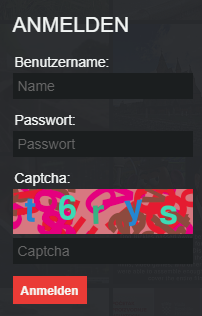
\includegraphics{gfx/mygraphics/pr0grammcaptcha.png}
    \caption{textbasiertes Captcha beim Login auf pr0gramm.com, das für Menschen mit Rot-Grün-Schwäche nur schwer zu erkennen ist}
    \label{fig:pr0grammcaptcha}
\end{figure}

\section{Technische Umsetzbarkeit}
\label{ch:matrix:tu}

Bei der technischen Umsetzbarkeit wird das Augenmerk auf die Implementation und Instandhaltung der Techniken gelegt. 
Unzureichende Dokumentation kann die Implementation und eventuelles Debugging erheblich erschweren 
und spielt deshalb eine wichtige Rolle bei der Auswahl. 

Ist die Dokumentation ausreichend? Werden viele Ressourcen benötigt? Muss man vorhandenen Quellcode stark abändern?

\section{Sicherheit}
\label{ch:matrix:sicherheit}
Sicherheit ist der Hauptgrund für die Verwendung von Spam-Präventionstechniken. 
Wie bereits in den vorherigen Kapiteln erwähnt, werden CAPTCHAs und ihre Alternativen genutzt um bei dem Ausfüllen von Formularen Bots auszusortieren
und somit Spam zu vermeiden.
Es muss betrachtet werden, ob es schon Methoden zur Umgehung der CAPTCHAs gibt. 
Gibt es sogar bereits künstliche Intelligenzen, die bestimmte Tests lösen können?

\section{Berechnung einer Metrik}
\label{ch:matrix:berechnung}
Bei der Berechnung einer Metrik auf Basis der entworfenen Matrix muss eine korrekte Gewichtung gewählt werden. 
Diese ist nötig, um individuelle Entscheidungen für unterschiedliche Einsatzgebiete treffen zu können,
da die Bedürfnisse dieser stark unterscheiden können. 

Die Gewichtung für jede Kategorie wird anteilig von 100 Prozent angegeben.
So wird es ermöglicht, präzise und individuell zu priorisieren.



